\documentclass[a4paper]{article}
\usepackage{float}
\usepackage[spanish,es-tabla]{babel}
\usepackage[T1]{fontenc}
\usepackage[spanish]{babel}
\usepackage{graphicx} 
\usepackage[utf8]{inputenc}
\usepackage{amsmath}
\usepackage{longtable}
\usepackage{graphicx}
\usepackage[colorinlistoftodos]{todonotes}
\usepackage[letterpaper,top=2.5cm,bottom=2.5cm,left=2cm,right=2cm,marginparwidth=2.5cm]{geometry}
\renewcommand{\baselinestretch}{1.25}


\title{Informe Física 4}
\author{Danny Córdova, Edwin Dávila}
\date{14 de Marzo del 2023}



\begin{document}

\maketitle

\section{Introducción}
En la presente práctica se revisó sobre uno de los pilares fundamentales de la física clásica: las tres Leyes de Newton. En la práctica se realizó un experimento en el cual se determinaron las tensiones de dos cuerdas y los coeficientes de rozamiento dinámico de un móvil con 10 masas diferentes. El objetivo principal de la práctica es usar los principios de la dinámica para poder calcular el valor del coeficiente de rozamiento de la mesa con el móvil.

\section{Metodología experimental}
Para las unidades de medida se usó el SI.  El tiempo se midió en segundos, la distancia en metros y la velocidad y aceleración con las respectivas unidades derivadas de metros y segundos. Para armar el experimento se siguió el siguiente esquema:

\begin{figure} [H]
    \centering
     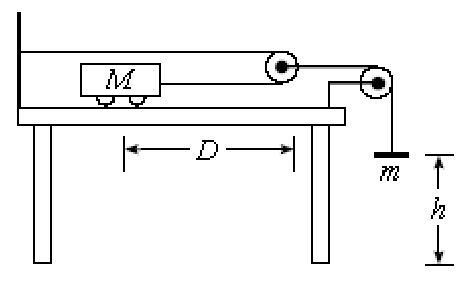
\includegraphics[width=0.4\textwidth]{Esquema del experimento 4.png}
    \caption{Esquema a seguir del experimento}
    \label{Esquema}
\end{figure}
Para el experimento de necesitó de 2 cuerdas con masa despreciable, 2 poleas, el móvil y un portamasas. El porta masas se colocó a una altura de 60 cm en todas las mediciones para poder hacer los cálculos sin fluctuaciones. A continuación se detallan las incertidumbres de los instrumentos de medida:
\begin{table}[H]
    \centering
    \begin{tabular}{|c|c|}
    \hline
        Balanza digital & $\pm1 g$ \\ \hline
        Cronómetro digital  & $\pm 0.5 s$ \\ \hline
        Regla láser  & $\pm 1 mm$ \\ \hline
    \end{tabular}
    \caption{Incertidumbre de los instrumentos de medida}
    \label{Incertidumbre de los instrumentos de medida}
\end{table}
Aunque el cronómetro digital tenga una incertidumbre verdadera de $\pm0.01 s$ debido al tiempo de reacción humano para prender y apagar el cronómetro se subió la incertidumbre al valor mostrado en la tabla. 

Se midieron un total de 10 masas diferentes, y para cada masa se midieron 10 tiempos con sus respectivos desplazamientos. Para el desplazamiento del móvil se tomó un valor fijo de 1.20 m debido a que la polea del móvil se movió el doble de la polea del portamasas.

Las variables directas que se midieron en el experimento son:
\begin{enumerate}
  \item Masa del móvil (M).
  \item Masa del portamasas (m).
  \item Altura del portamasas (h).
  \item Desplazamiento del móvil (D).
\end{enumerate}

Las variables indirectas que se calculan a partir de la información obtenida son:
\begin{enumerate}
  \item Aceleración del móvil y del porta masas($a_1$ y $a_2$).
  \item Tensión de la cuerda del móvil y del portamasas ($T_1$  y $T_2$).
 \item Coeficiente de rozamiento dinámico ($\mu_D$)
\end{enumerate}

Las fórmulas usadas en este experimento son:
\begin{equation}
    a=\frac{2D}{t^2}
\end{equation}
donde a es la aceleración en el intervalo de tiempo t y D es el desplazamiento(que puede cambiarse con la altura h para calcular la aceleración del portamasas). Esta fórmula solo se usa para MRU y cuando la $V_o$ y $x_o$ son 0.
\begin{equation}
    N=-mg
\end{equation}
donde N es la fuerza normal, m la masa y g la aceleración de la gravedad. Cabe aclarar que esta fórmula es solo una simplificación de la fórmula general pero que sirve para los casos en el que el plano no tiene inclinación. 

\begin{equation}
    F=ma
\end{equation}
donde F es la Fuerza total del sistema. En el caso en donde interactúa más de una fuerza se usa un sumatorio de fuerzas.

\begin{equation}
    \mu= \frac{\displaystyle\sum_{i=1}^{n} x_i}{n}
\end{equation}
donde $\mu$ es la media del conjunto $x_i$ y n el número de elementos del conjunto $x_i$.
 

\section{Resultados y observaciones}

Se ha tomado los tiempos de recorrido de $m$ con diferentes masas, de 100 g a 650 g, para los posteriores cálculos se tomara en cuenta la masa de el portamasas (50 g).


Se calcula el promedio de los tiempos para cada masa utilizando la fórmula (4) (para tiempos, consultar anexos). 

\

\

Se obtiene: 


\begin{table}[H]
\begin{center}
\begin{tabular}{|l|l|l|l|l|l|l|l|l|l|}
\hline
\textbf{100} & \textbf{150} & \textbf{200} & \textbf{250} & \textbf{300} & \textbf{350} & \textbf{400} & \textbf{450} & \textbf{500} & \textbf{650} \\ \hline
4,658        & 2,756        & 2,065        & 1,831        & 1,619        & 1,514        & 1,394        & 1,304        & 1,227        & 1,073        \\ \hline
\end{tabular}
\caption{Promedio de tiempo a diferentes $m$}
\end{center}
\end{table}

Ahora procedemos a calcular $a_1$ y $a_2$ mediante la fórmula (1):
Para la masa M (del móvil):
\[ a_1=\frac{2(1,2)}{t^2}\]
De manera similar, para la masa m (del portamasas):
\[ a_2= \frac{2(0,6)}{t^2}\]

\begin{table}[H]
\begin{center}
\begin{tabular}{|l|l|l|l|l|l|l|l|l|l|l|}
\hline
\textbf{} & \textbf{150} & \textbf{200} & \textbf{250} & \textbf{300} & \textbf{350} & \textbf{400} & \textbf{450} & \textbf{500} & \textbf{550} & \textbf{700} \\ \hline
$a_1$         & 0,111        & 0,316        & 0,563        & 0,716        & 0,916        & 1,047        & 1,235        & 1,411        & 1,594        & 2,085        \\ \hline
$a_2$         & 0,055        & 0,158        & 0,281        & 0,358        & 0,458        & 0,524        & 0,618        & 0,706        & 0,797        & 1,042        \\ \hline
\end{tabular}
\caption{Aceleraciones de cada cuerpo a variante $m$}
\end{center}
\end{table}

De donde rescatamos la gráfica de la aceleración en función de la masa:
\begin{figure} [H]
    \centering
    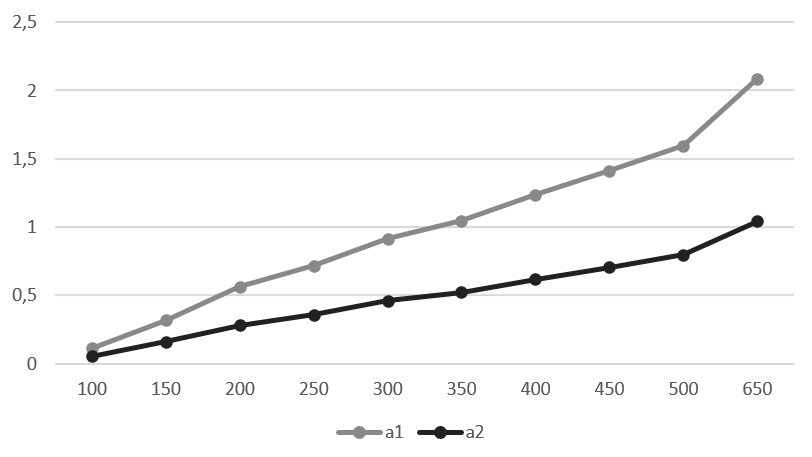
\includegraphics[width=0.55\textwidth]{Gráfico aceleración vs masa.png}
    \caption{Aceleración en función de la masa}
    \end{figure}
\

\

\

\

\

\

\

\

\

Se tiene los siguientes diagramas de cuerpo libre: 
\begin{figure} [H]
    \centering
    \includegraphics[width=0.35\textwidth]{Diagrama de cuerpo libre del móvil.png}
    \caption{Diagrama de cuerpo libre del móvil}
    \end{figure}
\begin{figure} [H]
    \centering
    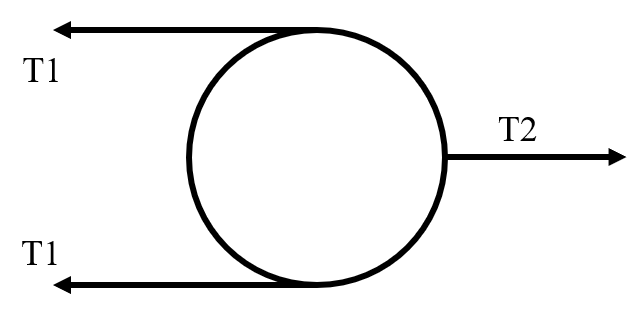
\includegraphics[width=0.35\textwidth]{Diagrama de las tensiones.png}
    \caption{Diagrama de las tensiones}
    \end{figure}
\begin{figure} [H]
    \centering
    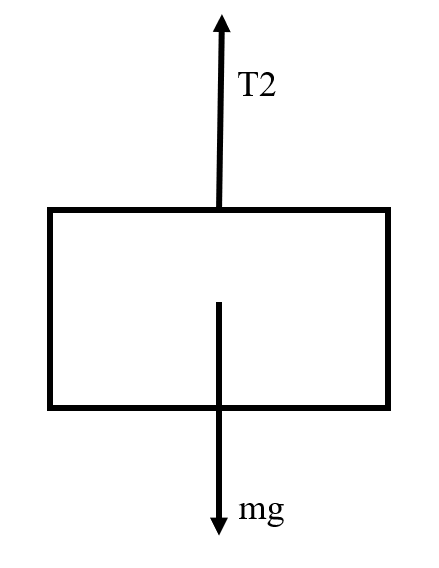
\includegraphics[width=0.2\textwidth]{Diagrama de cuerpo libre del portamasas.png}
    \caption{Diagrama de cuerpo libre del portamasas}
    \end{figure}

Partiendo del diagrama de cuerpo libre se tiene que para el móvil: 

\[ \sum{Fy} \Rightarrow N=Mg\]
\[ \sum {Fx} \Rightarrow T1-fr=Ma_1\]

Obteniendo así el coeficiente de rozamiento de la mesa  $\mu$:

\[\mu= \frac{T1-Ma_1}{Mg}\]

Observando la polea móvil se sabe que:

\[T2=2(T1)\]

Analizando el diagrama de cuerpo libre de m, se tiene que:

\[\sum{Fy} \Rightarrow mg-T2=ma_2\]
\[T2=m(g-a_2)\]
Deduciendo así $T1$:

\[T1= \frac{m(g-a_2)}{2}\]

Procedemos ahora a calcular T1, T2 y $\mu$ considerando cada dato de masa añadiendo la masa del portamasas:

\begin{table}[H]
\begin{center}
\begin{tabular}{|l|l|l|l|l|l|l|l|l|l|l|}
\hline
\textbf{} & \textbf{150} & \textbf{200} & \textbf{250} & \textbf{300} & \textbf{350} & \textbf{400} & \textbf{450} & \textbf{500} & \textbf{550} & \textbf{700} \\ \hline
T1         & 0,729        & 0,962        & 1,186        & 1,412        & 1,630        & 1,850        & 2,060        & 2,267        & 2,468        & 3,056        \\ \hline
T2         & 1,458        & 1,923        & 2,373        & 2,825        & 3,260        & 3,700        & 4,120        & 4,534        & 4,937        & 6,112        \\ \hline
$\mu$         & 0,050        & 0,048        & 0,042        & 0,045        & 0,043        & 0,048        & 0,046        & 0,045        & 0,044        & 0,043        \\ \hline
\end{tabular}
\caption{Aceleraciones de cada cuerpo a variante $m$}
\end{center}
\end{table}

Para finalizar calculamos el promedio de $\mu$:
\[ \mu=\frac{\displaystyle\sum_{i=1}^{10} \mu_i}{10}= 0,0453\]
\section{Conclusiones}

Gracias al experimento se puede observar una relación directa entre masa y aceleración, mientras más masa tenía el portamasas menos tiempo se demoraba el móvil en recorrer la distancia de 1.20m. Además, de esto, se pudo calcular el valor del coeficiente de fricción con la mesa. No se conoce cuál es el valor real de dicho coeficiente ya que no se tenía un coeficiente de referencia, sin embargo, puede existir un error considerable debido a la incertidumbre elevada del tiempo de reacción humano en encender y apagar el cronómetro debido al corto tiempo que le tomaba al móvil recorrer lo establecido. 

\section{Anexos}
\begin{table}[H]
\begin{center}
\begin{tabular}{|c|c|c|c|c|c|c|c|c|c|}
\hline
\textbf{100} & \textbf{150} & \textbf{200} & \textbf{250} & \textbf{300} & \textbf{350} & \textbf{400} & \textbf{450} & \textbf{500} & \textbf{650} \\ \hline
4,52         & 2,81         & 1,91         & 1,72         & 1,61         & 1,54         & 1,35         & 1,27         & 1,19         & 1,12         \\ \hline
4,79         & 2,89         & 2,19         & 1,78         & 1,71         & 1,47         & 1,44         & 1,31         & 1,24         & 1,06         \\ \hline
4,67         & 2,67         & 1,89         & 1,83         & 1,62         & 1,54         & 1,38         & 1,34         & 1,22         & 1,01         \\ \hline
4,78         & 2,85         & 1,97         & 1,85         & 1,57         & 1,55         & 1,36         & 1,33         & 1,18         & 1,13         \\ \hline
4,54         & 2,58         & 1,88         & 1,71         & 1,65         & 1,48         & 1,39         & 1,31         & 1,26         & 1,09         \\ \hline
4,52         & 2,63         & 2,23         & 1,98         & 1,68         & 1,49         & 1,34         & 1,28         & 1,22         & 1,05         \\ \hline
4,52         & 2,72         & 2,12         & 1,92         & 1,58         & 1,53         & 1,44         & 1,26         & 1,19         & 1,08         \\ \hline
4,79         & 2,84         & 2,21         & 1,68         & 1,63         & 1,48         & 1,46         & 1,32         & 1,27         & 1,07         \\ \hline
4,67         & 2,74         & 2,11         & 1,93         & 1,59         & 1,54         & 1,41         & 1,28         & 1,22         & 1,03         \\ \hline
4,78         & 2,83         & 2,14         & 1,91         & 1,55         & 1,52         & 1,37         & 1,34         & 1,28         & 1,09         \\ \hline
\end{tabular}
\caption{Tiempos de recorrido del portamasas a diferentes $m$}
\end{center}
\end{table}

\end{document}
